\section{Method}\label{sec:method}
\paragraph{Pieces and paths.} A piece is a regular polygon $P$ with unit side and inradius $\rho$ (a unit square, triangle or hexagon), or a unit-diameter disk. Its \emph{shape state} is
\[
P(\gamma,\tau)=\gamma\big[(1-\tau)\,P\;\oplus\;\tau\rho\,D\big],
\]
the polygon scaled about its incenter, dilated by a disk of radius $\tau\rho$ (a spheropolygon \citep{AlonsoMarroquin2008}), and scaled by $\gamma$. At $\tau=1$ it is the inscribed disk, at $\tau=0$ the polygon, and for $\gamma\le1$ every state lies inside the polygon, so moving toward $(\gamma,\tau)=(1,0)$ only grows the piece. Two facts describe what the family does. Its support function is
\[
h_{P(\gamma,\tau)}(u)=\gamma\big[(1-\tau)\,h_P(u)+\tau\rho\big],
\]
for a unit direction $u$, so the dependence of a piece's extent on its orientation is scaled down by $(1-\tau)$: rotating a nearly round piece barely changes the energy, and orientation becomes a decision only late in the path. And since $A(P)=\tfrac12\,\mathrm{perimeter}\cdot\rho$, its area at $\gamma=1$ is
\[
A(\tau)=A(P)-\big[A(P)-\pi\rho^2\big]\tau^2 ,
\]
so a hardening piece gains the area outside its inscribed disk, $21\%$ of a square, $9\%$ of a hexagon and $40\%$ of a triangle. A \emph{path} is a schedule for $(\gamma,\tau)$ during the middle phase of a run (Figure~\ref{alg:run}). We compare three:
\begin{itemize}\itemsep0pt
\item \textbf{harden}: $\gamma=1$, $\tau:1\to0$ (disks harden into polygons);
\item \textbf{grow}: $\tau=0$, $\gamma:\gamma_0\to1$ (rigid polygons grow, as in Lubachevsky--Stillinger \citep{lubachevsky});
\item \textbf{rigid}: $(\gamma,\tau)=(1,0)$ throughout, on the same schedule;
\end{itemize}
and two classical baselines on rigid pieces: \textbf{sa}, Metropolis simulated annealing over poses and container size \citep{kirkpatrick}, and \textbf{pc}, perturbation--compression \citep{Gensane2004,gensane} (shrink, relax, perturb on failure). Two further paths serve as ablations: \textbf{snap} compresses disks exactly as harden does and then switches to the polygons at once ($\tau:1\to0$ in one step), and \textbf{grow-area} keeps rigid polygons whose area follows hardening's area schedule ($\tau=0$, $\gamma^2=1-(1-\pi\rho^2/A)\,t^2$ with $t:1\to0$).

\paragraph{Energy.} The container (square, equilateral triangle or circle) is centred at the origin with size $L$: side length for a square/equilateral triangle, radius for a circle. For poses $(x_i,y_i,\theta_i)$,
\[
E=\sum_{i<j}\big(2r-\operatorname{sd}_{ij}\big)_+^2+\sum_{i}\sum_{v}\big(\text{wall violation of }v\big)_+^2+\mu L,
\]
where $r=\gamma\tau\rho$, $\operatorname{sd}_{ij}$ is the signed distance between the cores (exact vertex--edge distance when apart, minus the separating-axis penetration depth when overlapping) and $v$ ranges over core vertices. The term $\mu L$ is inward pressure. Positions, angles and $L$ follow momentum gradient descent with analytic gradients and decaying Gaussian noise. In 3D the same holds for cubes with quaternion orientations and the 15-axis separating test \citep{softtorigidpacking}.

\begin{figure}[t]
\centering\fbox{\begin{minipage}{0.92\linewidth}\small
\textbf{One gradient-path run.} Let $B$ denote the budget multiplier; base compression, morph and settling lengths are $n_C,n_M,n_S=2500,7500,1500$ steps.
\begin{enumerate}\itemsep0pt
\item Initialize random poses in a container of area $3.2$ times the pieces' area; set $(\gamma,\tau)$ to the path start.
\item Compress for $Bn_C$ steps with pressure $3\mu$ and decaying noise.
\item Follow the path for $Bn_M$ steps: update $(\gamma,\tau)$ with normalized progress, and take momentum steps at pressure $\mu$ with decaying noise.
\item Settle the final pieces for $Bn_S$ steps with no noise, decaying pressure as $\mu 10^{-4s/(Bn_S)}$.
\item Legalise by scaling centres apart until the pair-overlap tolerance is met, then measure the smallest container.
\end{enumerate}
\end{minipage}}
\caption{One gradient-path run with the step schedule used in the study}\label{alg:run}
\end{figure}

\paragraph{Step details.} Each momentum step updates velocities as $v\leftarrow0.85\,v-0.04\,\nabla E$ (container size: $v_L\leftarrow0.85\,v_L-0.02\,(\mu+\partial E/\partial L)$), caps a piece's translation step at $0.03\sqrt2\,R$ ($R$ the circumradius) and its rotation at $0.03$ rad, then adds Gaussian noise. With noise multiplier $\nu$ (Appendix, frozen settings), the positional noise is $0.015\,\nu\,(1-u)$ during compression and $0.004\,\nu\,(1-u)$ during the path, where $u\in[0,1]$ is progress through the phase, and the angular noise is $1.5$ times the positional noise. The implementation is \texttt{engine/engine2d.js}.

\begin{figure}[t]\centering
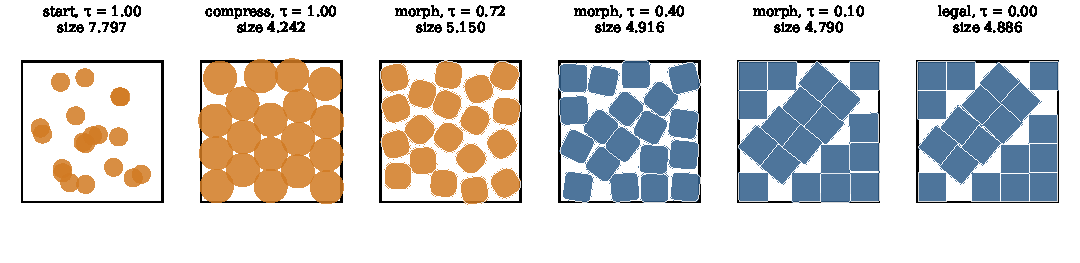
\includegraphics[width=\linewidth]{figures/strip_squ19}\\[2pt]
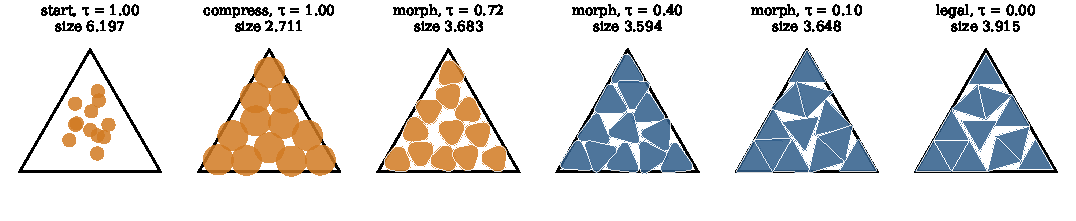
\includegraphics[width=\linewidth]{figures/strip_tri12}
\caption{Two hardening runs (C07). Top: 19 squares; disks are compressed, harden into squares, and settle into Wainwright's packing (side $3+4\sqrt2/3$), which no other method reached in 32 runs. Bottom: the best of 32 hardening runs for 12 triangles in a triangle ends at $3.915$, while rigid and snap starts reach the best known $3.879$; the triangles that emerge from the near-hexagonal disk arrangement keep orientations that do not tile. These are selected decimated replays from versioned campaign files. The triangle size $3.915$ is the legalised simulator endpoint before tightening.}\label{fig:strip}\label{fig:tristrip}
\end{figure}

\paragraph{Legalisation, tightening and certification scope.} Penalties tolerate small overlaps, so every run is \emph{legalised}: centres are scaled apart about their mean until no pair overlaps by more than $10^{-12}$ under the separating-axis test, and the smallest container (translation free) is measured. Near-best runs are then \emph{tightened} by constrained numerical optimisation: minimise $L$ over poses and one separating line (plane) per nearby pair \citep{Peralta2018}, with every vertex inside the container, by SLSQP \citep{kraft} in trust-region outer iterations, keeping a step only if the independently legalised size decreases. Tightening is a local method and gives no optimality guarantee; it only removes the slack a penalty method leaves. The below-catalogue certification route (not applied to every numerically reached catalogue value) spreads a tightened packing below a catalogue value to a clearance of $10^{-6}$ and checks it twice: in floating point, and in exact rational arithmetic. The exact check uses rational rotations from $\tan(\theta/2)$, replaces each piece by a rational polygon scaled by $1+10^{-8}$ and proves, in $\mathbb{Q}(\sqrt3)$, that this polygon contains the true unit polygon with margin $10^{-9}$, and exhibits a rational separating direction for every pair. The current exact 2D checker supports circles, triangles, squares and hexagons; it does not certify the pentagon/octagon families in C15. A numeric reached classification is not an exact certificate or an optimality proof. No below-catalogue claim folder was produced by this controlled study. Online Resource~1 checks four separately enlarged square witnesses; those certificates do not establish feasibility at their original contact objectives.

\paragraph{Budgets.} A run's budget is its number of steps: every gradient path takes $11{,}500\,B$ steps. Pair evaluations then differ by path, since soft pieces have more near neighbours: at $n=20$ squares in a square a hardening run makes about $1.2\times$ the pair evaluations of a rigid run (Table~\ref{tab:diag} in the appendix), which, if anything, favours hardening. The two baselines are stopped once their pair evaluations exceed those of a reference hardening run at the same $n$ (one fixed seed, with the baseline's own pressure and noise settings); for squares in a square this reference is \RefEvalsTwenty{} pair evaluations at $n=20$ and \RefEvalsThirty{} at $n=30$, $\RefRatioTwenty$ and $\RefRatioThirty$ times the mean of the 32 tuned hardening runs. Simulated annealing adds a final short gradient relaxation; perturbation--compression stops at the end of a relaxation. For the square-in-square diagnostics in Table~\ref{tab:diag}, mean pair evaluations divided by the saved reference allowance are $1.02476$ and $1.02520$ for annealing at $n=20,30$, respectively, and $1.57588$ and $1.68891$ for perturbation--compression. These are means for those two cells, not global maxima. In recorded simulator wall-clock time on one core of the study machine (Node.js; tightening excluded), hardening was the fastest of the five methods in the two square-in-square diagnostic cells, $n=20$ and 30 (Table~\ref{tab:diag}). This timing observation is specific to the measured machine and simulator workload. It excludes tuning, repeated reference runs, postprocessing and verification, so it does not establish equal end-to-end cost or general wall-clock superiority.

\paragraph{Endpoint and assistance definitions.} For non-truncated values, a run reaches the catalogue when its selected size is no more than the value plus $10^{-9}$. For truncated values, the ledger verdict uses a gap strictly below the stored printed-precision tolerance (default $10^{-5}$), while the later saved statistical/policy code uses size no greater than value plus tolerance. Lowest-size ties use relative $10^{-9}$, with an additional $10^{-12}$ absolute allowance in the C07 descriptive count code; C15 strict-lower comparisons use $x<y(1-10^{-9})$. These numeric rules do not certify equality or optimality. Substantive AI assistance in implementation, analysis, writing and preparation review is described in Statements and Declarations.
